\loesung{
\begin{enumerate} [a)]
  \item Derivation of PD function for $S = \{1\}$ (with $C = \{2\}$) given
  \begin{equation*}
   \fh(\xv) = \fh(x_1, x_2) = \hat\beta_1 x_1 + \hat\beta_2 x_2 + \hat\beta_3 x_1 x_2 + \hat\beta_0
  \label{eq:linmod}
  \end{equation*}
  
  $$
  \begin{aligned}
  f_{1, PD}(x_1) = \E_{x_2} \left( \fh(x_1, x_2) \right) &= \int_{-\infty}^{\infty} \left( \hat\beta_1 x_1 + \hat\beta_2 x_2 + \hat\beta_3 x_1 x_2 + \hat\beta_0 \right) \, d\P(x_2) \\
  &= \hat\beta_1 x_1 + \int_{-\infty}^{\infty} \hat\beta_2 x_2 + \hat\beta_3 x_1 x_2 \, d\P(x_2) + \hat\beta_0 \\
    &= \hat\beta_1 x_1 + \int_{-\infty}^{\infty} (\hat\beta_2 + \hat\beta_3 x_1) x_2 \, d\P(x_2) + \hat\beta_0 \\
    &= \hat\beta_1 x_1 + (\hat\beta_2 + \hat\beta_3 x_1) \cdot \int_{-\infty}^{\infty} x_2 \, d\P(x_2) + \hat\beta_0 \\
        &= \hat\beta_1 x_1 + (\hat\beta_2 + \hat\beta_3 x_1) \cdot \E_{x_2} (x_2) + \hat\beta_0 
  \end{aligned}
  $$

  \item PD function for $\hat\beta_0 = 0$, $\hat\beta_1 = -8$, $\hat\beta_2 = 0.2$, $\hat\beta_3 = 16$, $X_1 \sim Unif(-1, 1)$ and  $X_2 \sim B(1, 0.5)$. 
  $$
  \begin{aligned}
  f_{1, PD}(x_1) = \hat\beta_1 x_1 + (\hat\beta_2 + \hat\beta_3 x_1) \cdot \E_{x_2} (x_2) + \hat\beta_0 
        &= -8 x_1 + (0.2 + 16 x_1) \cdot \E_{x_2} (x_2) + 0 \\
        &= -8 x_1 + (0.2 + 16 x_1) \cdot 0.5 \\
        &= -8 x_1 + 0.1 + 8 x_1 \\
        &= 0.1 %+ 0 x_1
  \end{aligned}
  $$
  
  \item ICE functions for group $X_2 = 1$ and for group $X_2 = 0$: 
    $$f_1(x_1) = \begin{cases}
      - 8 x_1 + (0.2 + 16 x_1) \cdot 1 = 8 x_1 + 0.2 & x_2 = 1 \\
      - 8 x_1 + (0.2 + 16 x_1) \cdot 0 = - 8 x_1 & x_2 = 0
    \end{cases}$$
    
  The light green dots correspond to group $X_2 = 1$, the light blue dots to group $X_2 = 0$.
  
   \item
   The example illustrates that by the averaging of ICE curves for a PD plot we might obfuscate heterogeneous effects and interactions. 
   Although the ICE curves here show a strong effect of $X_1$ on $Y$, the effect is not apparent in the PDP.
   Therefore, it is highly recommended to plot PD plots and ICE curves together. 

\begin{center}
  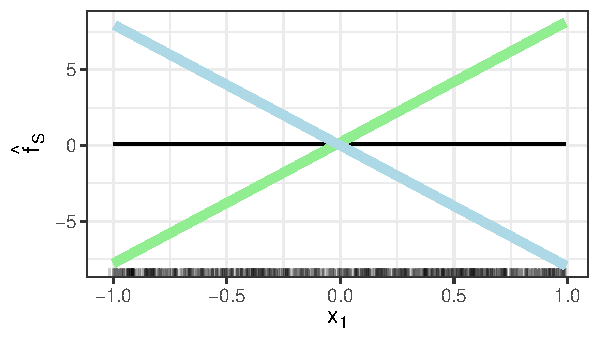
\includegraphics[width=\maxwidth]{figure/pdpinteraction_ICE_curve_sol.pdf}
\end{center}

  
\end{enumerate}
}